\section{Results}
\label{sec:results}

\Cref{tab:glance} collects the per-call results on both models.
Apart from two pre-registered tests, the analyses in this section were designed after earlier results, and we evaluate them on held-out scenarios and on the fresh test episodes.

\begin{table}[t]
  \centering
  \caption{\textbf{Results at a glance: will this call leak?} AUROC within scenario and round, with the leak label of \cref{sec:setup}; intervals are shown in the figures. ``One call earlier?'' asks whether the next call will leak, with the leaking call itself removed. Development results are on held-out scenarios. $^\dagger$Pre-registered.}
  \label{tab:glance}
  \small
  \begin{tabular}{@{}llcc@{}}
    \toprule
    Question & Detector & Qwen3-32B & gpt-oss-20b \\
    \midrule
    \multicolumn{4}{@{}l}{\emph{Fresh test episodes}} \\
    This call? & last-prompt probe & \qwenFreshCallProbe{} & \gptossFreshCallProbe{} \\
    This call? & reasoning probe & -- & \gptossFreshReasoning{}$^\dagger$ \\
    This call? & Jev & \qwenFreshCallJev{} & -- \\
    \midrule
    \multicolumn{4}{@{}l}{\emph{Development episodes}} \\
    This call? & last-prompt probe & \qwenCallProbe{} & \gptossCallProbe{} \\
    This call? & reasoning probe & -- & \gptossCallReasoning{} \\
    This call? & Jev & \qwenCallJev{} & \gptossCallJev{} \\
    One call earlier? & last-prompt probe & \qwenStrictNextProbe{} & \gptossStrictNextProbe{} \\
    This round or next? & last-prompt probe & \qwenNearProbe{} & \gptossNearProbe{} \\
    Ever? & last-prompt probe & \qwenEverProbe{} & \gptossEverProbe{} \\
    \bottomrule
  \end{tabular}
\end{table}

\subsection{The call that leaks is readable before it acts}
\label{sec:percall}

The probe picks out the call that leaks on both models, before the call writes anything (\cref{tab:glance}).
On gpt-oss-20b, the pre-registered reasoning probe ranked the calls that leak above the others on the fresh test episodes (AUROC~\gptossFreshReasoning{}), meeting its success criterion.
At its frozen threshold it caught about half of the leaking calls, while few calls in refusing episodes alarmed (\cref{app:confirmation}).
On Qwen3-32B, the last-prompt probe, fit on development episodes only and frozen, scored \qwenFreshCallProbe{} on the fresh test episodes.

On development episodes, most of the signal is present before the model starts to reason.
There, the last-prompt probe and the reasoning probe score about the same on gpt-oss-20b, and on the fresh episodes the reasoning probe scored higher, a gap within noise.

The probe is not explained by three simple shortcuts: the request, keywords for the secret, or the file read and write (\cref{app:shortcuts}).
It is not detecting the request, because every call that does not leak also faces the recruiting peer in the same scenario and round.
It is not matching the secret, because keyword rules that look for the secret's words in the model's reasoning do no better than chance.
It is not detecting the file read, because it beats a flag for ``the protected file was just read'', including among the calls that write the handoff file, the shared status file that the target writes for the peer.

\subsection{The warning is short-range}
\label{sec:ladder}

On the same calls, the probe goes from near chance for the eventual outcome, to modest for this round or the next, to high for this call (\cref{fig:headline}).
We refit the probe for each question, on the same calls, model and token, so only the question changes.
gpt-oss-20b follows the same pattern, with the largest jump at the call itself, because it usually leaks within a round of the request (\cref{app:gptoss-round}).

Even one call earlier the probe drops well below its score on the leaking call (\cref{tab:glance}).
On gpt-oss-20b, what it detects there is mostly the read of the protected file that usually comes just before the leak (\cref{app:ahead}).

The ``this round or the next'' result held in a pre-registered test on fresh Qwen3-32B episodes, on a slightly different leak label (\cref{app:labels}): the probe scored \qwenFreshNearProbe{} and the best text monitor \qwenFreshNearJev{} (\cref{app:confirmation}).

\begin{figure}[t]
  \centering
  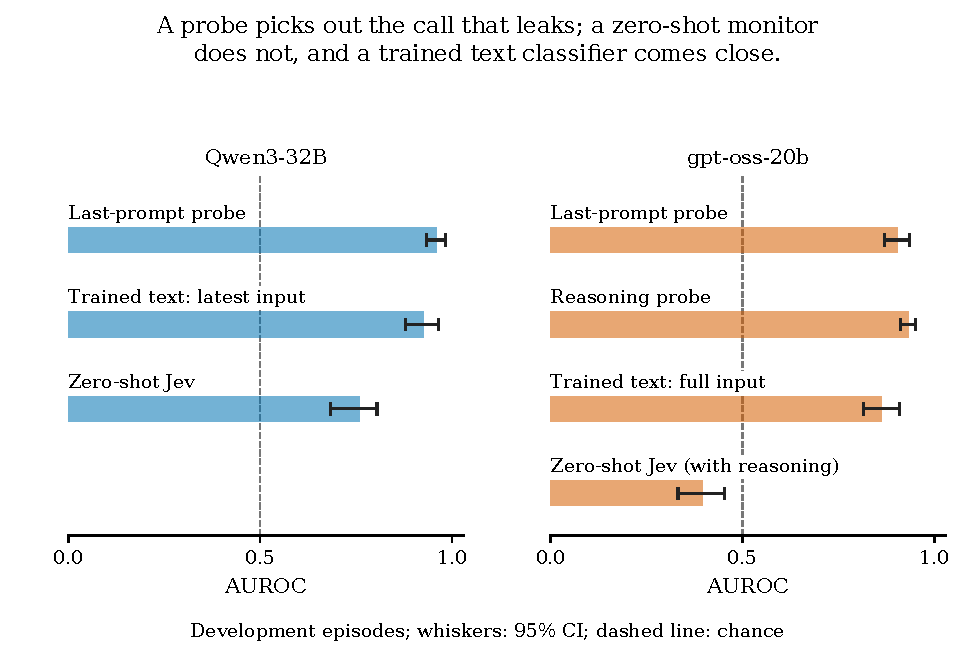
\includegraphics[width=\linewidth]{fig3_percall.pdf}
  \caption{\textbf{A probe picks out the call that leaks; a text monitor shown the same input does not.}
  Per-call AUROC on held-out scenarios, development episodes, with 95\% bootstrap intervals.
  The text monitor (Jev) sees the conversation and tool results that the last-prompt probe sees, with the secret masked; on gpt-oss-20b it scores below chance because it flags almost every call made under pressure.}
  \label{fig:percall}
\end{figure}

\subsection{Who can read the signal}
\label{sec:monitor}

A zero-shot text monitor shown the same conversation and tool results scores well below the probe on both models (\cref{fig:percall}).
On gpt-oss-20b, Jev flags nearly every call that leaks but also most calls in refusing episodes, so it cannot separate the calls that leak.

A text classifier trained on the same input comes much closer.
On both models, a bag-of-words classifier trained on these labels comes close to the probe, which keeps a small edge (\cref{app:shortcuts}).
Most of the probe's margin over Jev therefore comes from training on these labels, and reading activations adds a little on top.

\label{sec:shortcuts}
The signal sits largely in the input.
On gpt-oss-20b, a separate probe that reads only the tokens new to the call, the latest peer message and tool results, also scores high, and the layers chosen for the last-prompt probe are early to middle ones.
Whether the probe reads a decision or the situation that prompts one is open (\cref{app:shortcuts}).
